\documentclass[letterpaper]{article}
\usepackage[margin=1in]{geometry}
\usepackage[utf8]{inputenc}
\usepackage{textcomp}
\usepackage{amssymb}
\usepackage{natbib}
\usepackage{graphicx}
\usepackage{gensymb}
\usepackage{amsthm, amsmath, mathtools}
\usepackage[dvipsnames]{xcolor}
\usepackage{enumerate}
\usepackage{mdframed}
\usepackage[most]{tcolorbox}
\usepackage{csquotes}
% https://tex.stackexchange.com/questions/13506/how-to-continue-the-framed-text-box-on-multiple-pages

\tcbuselibrary{theorems}

\newcommand{\R}{\mathbb{R}}
\newcommand{\Z}{\mathbb{Z}}
\newcommand{\N}{\mathbb{N}}
\newcommand{\Q}{\mathbb{Q}}
\newcommand{\C}{\mathbb{C}}
\newcommand{\code}[1]{\texttt{#1}}
\newcommand{\mdiamond}{$\diamondsuit$}
\newcommand{\PowerSet}{\mathcal{P}}
\newcommand{\Mod}[1]{\ (\mathrm{mod}\ #1)}
\DeclareMathOperator{\lcm}{lcm}

%\newtheorem*{theorem}{Theorem}
%\newtheorem*{definition}{Definition}
%\newtheorem*{corollary}{Corollary}
%\newtheorem*{lemma}{Lemma}
\newtheorem*{proposition}{Proposition}


\newtcbtheorem[number within=section]{theorem}{Theorem}
{colback=green!5,colframe=green!35!black,fonttitle=\bfseries}{th}

\newtcbtheorem[number within=section]{definition}{Definition}
{colback=blue!5,colframe=blue!35!black,fonttitle=\bfseries}{def}

\newtcbtheorem[number within=section]{corollary}{Corollary}
{colback=yellow!5,colframe=yellow!35!black,fonttitle=\bfseries}{cor}

\newtcbtheorem[number within=section]{lemma}{Lemma}
{colback=red!5,colframe=red!35!black,fonttitle=\bfseries}{lem}

\newtcbtheorem[number within=section]{example}{Example}
{colback=white!5,colframe=white!35!black,fonttitle=\bfseries}{def}

\newtcbtheorem[number within=section]{note}{Important Note}{
        enhanced,
        sharp corners,
        attach boxed title to top left={
            xshift=-1mm,
            yshift=-5mm,
            yshifttext=-1mm
        },
        top=1.5em,
        colback=white,
        colframe=black,
        fonttitle=\bfseries,
        boxed title style={
            sharp corners,
            size=small,
            colback=red!75!black,
            colframe=red!75!black,
        } 
    }{impnote}
\usepackage[utf8]{inputenc}
\usepackage[english]{babel}
\usepackage{fancyhdr}
\usepackage[hidelinks]{hyperref}

\pagestyle{fancy}
\fancyhf{}
\rhead{MATH 155A}
\chead{Tuesday, March 29, 2022}
\lhead{Lecture 1}
\rfoot{\thepage}

\setlength{\parindent}{0pt}

\begin{document}

\section{Three Paradigms for Rendering}
We first begin by discussing how to render points, lines, and triangles. 

\subsection{Drawing Points}
Consider the following graph:
\begin{center}
    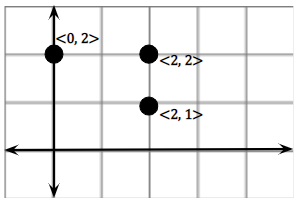
\includegraphics[scale=1]{../assets/points1.png}
\end{center}
In this class, we represent points in the form $\cyclic{x, y}$, or $\begin{bmatrix}
    x \\ y
\end{bmatrix}$. In C++, we can represent these points like so: 
\begin{verbatim}
    float verts[][2] = {
        {2, 1},
        {2, 2},
        {0, 2}
    };\end{verbatim}
After loading the array into the GPU, which we'll discuss later, we can use a command like: 
\begin{verbatim}
    glDrawArrays(GL_POINTS, 0, 3);\end{verbatim}

\subsection{Drawing Lines}
Consider the following graph:
\begin{center}
    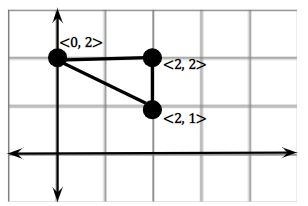
\includegraphics[scale=1]{../assets/line1.png}
\end{center}
In JavaScript, we can make use of the Canvas API to draw this like so: 
\begin{verbatim}
    moveTo(2, 1);
    lineTo(2, 2);
    lineTo(0, 2);
    lineTo(2, 2);
    stroke();\end{verbatim}
In OpenGL, we would do something like: 
\begin{verbatim}
    glDrawArrays(GL_LINE_LOOP, 0, 3);\end{verbatim}
The \code{GL\_LINE\_LOOP} means that we're making a closed loop of edges, using 3 vertices in total. 

\bigskip 

There are several other modes that we can use. To see how these differ, we'll use the following set of vertices as an example:
\begin{center}
    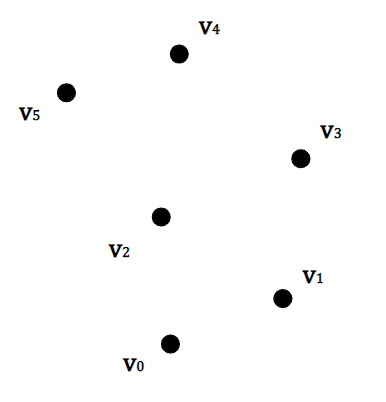
\includegraphics[scale=0.5]{../assets/points2.png}
\end{center}
\begin{itemize}
    \item \code{GL\_LINES}: If we have the following code segment
    \begin{verbatim}
        glDrawArrays(GL_LINES, 0, 6);\end{verbatim}
    Then, we would get the following drawing:
    \begin{center}
        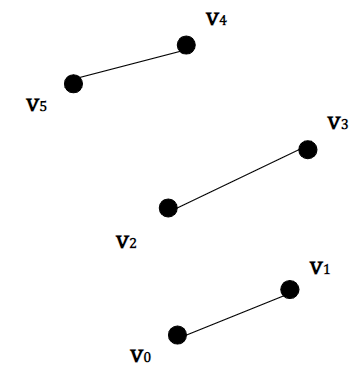
\includegraphics[scale=0.5]{../assets/points3.png}
    \end{center}

    \item \code{GL\_LINE\_STRIP}: Now, if we were to include the following code segment in addition to the one above
    \begin{verbatim}
        glDrawArrays(GL_LINES_STRIP, 0, 6);\end{verbatim}
    Then, we would get the following drawing: 
    \begin{center}
        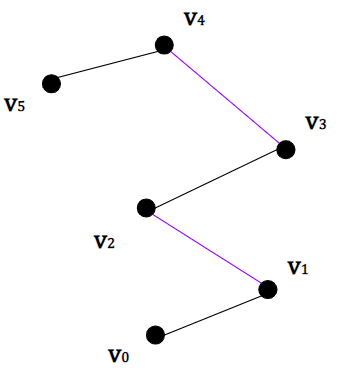
\includegraphics[scale=0.5]{../assets/points4.png}
    \end{center}

    \item \code{GL\_LINE\_LOOP}: Finally, including 
    \begin{verbatim}
        glDrawArrays(GL_LINES_LOOP, 0, 6);\end{verbatim}
    would yield the following drawing: 
    \begin{center}
        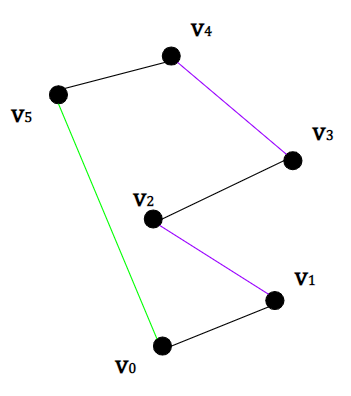
\includegraphics[scale=0.5]{../assets/points5.png}
    \end{center}
\end{itemize}


So, to sumamrize, if we have the vertices $\{v_1, v_2, \dots, v_n\}$, then: 
\begin{itemize}
    \item \code{GL\_LINES} will draw a line for each pair of vertices; that is, a line will be drawn between $v_1$ and $v_2$, $v_3$ and $v_4$, and so on. 
    \item \code{GL\_LINE\_STRIP} will draw a line for each consecutive pair of vertices, up to and including $v_{n - 1}$; that is, a line will be drawn between $v_1$ and $v_2$, $v_2$ and $v_3$, $v_3$ and $v_4$, and so on. The last line drawn will be from $v_{n - 1}$ to $v_{n}$. 
    \item \code{GL\_LINE\_LOOP} will draw a line for each consecutive pair of vertices, including from the end vertex to the start vertex. So, effectively, this is just \code{GL\_LINE\_STRIP} but with a line from $v_n$ to $v_1$.  
\end{itemize}

\subsection{Drawing Triangles}
Like with drawing lines, there are three modes for drawing triangles. 
\begin{itemize}
    \item \code{GL\_TRIANGLES}
    \item \code{GL\_TRIANGLE\_FAN}
    \item \code{GL\_TRIANGLE\_STRIP}
\end{itemize}
Using the same set of 6 points above, we show the following examples. 

\subsubsection{\code{GL\_TRIANGLES} Mode}
This mode groups the vertices into groups of three, and then draws a triangle between each group. For example, if you have vertices $\{v_0, \dots, v_5\}$, then this mode would take vertices $\{v_0, \dots, v_2\}$ and $\{v_3, \dots, v_5\}$ and draw a triangle (from $v_0 \to v_1$ and then from $v_1 \to v_2$ and finally $v_2 \to v_0$, while filling it in with a color).

\bigskip 

When we use the \code{GL\_TRIANGLES} mode, like so: 
\begin{verbatim}
    glDrawArrays(GL_TRIANGLES, 0, 6);
\end{verbatim}
Then we get something like: 
\begin{center}
    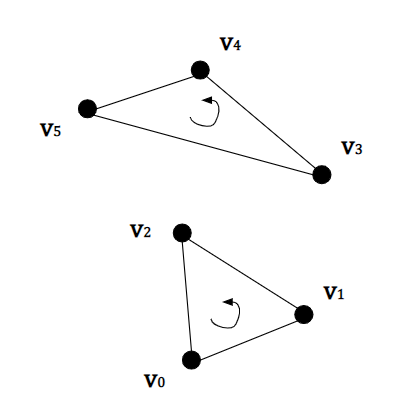
\includegraphics[scale=0.5]{../assets/triangle1.png}
\end{center}
Note that the arrows here indicate that we're looking at the ``front'' faces of the triangle. The ``back'' face is the other side. 

\subsubsection{\code{GL\_TRIANGLE\_FAN} Mode}
For an array of vertices $\{v_0, \dots, v_n\}$, $v_0$ is the common vertex. Then, the rest of the vertices $v_1, \dots, v_n$ are defining a triangle which shares the initial vertex.

\bigskip

Suppose you're given the following set of vertices like so: 
\begin{center}
    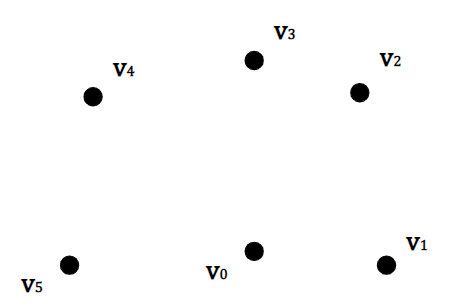
\includegraphics[scale=0.5]{../assets/triangle2.png}
\end{center}

When using this mode, like so 
\begin{verbatim}
    glDrawArrays(GL_TRIANGLE_FAN, 0, 6);
\end{verbatim}
Then we get something like: 
\begin{center}
    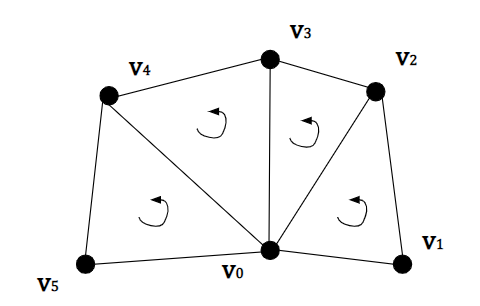
\includegraphics[scale=0.5]{../assets/triangle3.png}
\end{center}

\subsubsection{\code{GL\_TRIANGLE\_STRIP} Mode}
Suppose you're given the following set of vertices like so: 
\begin{center}
    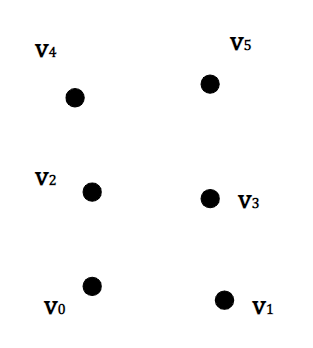
\includegraphics[scale=0.5]{../assets/triangle4.png}
\end{center}

When using this mode, like so 
\begin{verbatim}
    glDrawArrays(GL_TRIANGLE_STRIP, 0, 6);
\end{verbatim}
Then we get something like: 
\begin{center}
    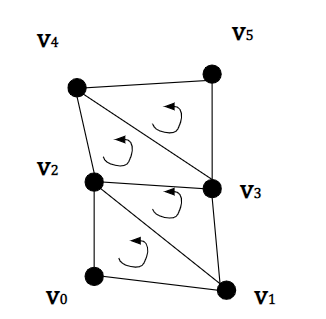
\includegraphics[scale=0.5]{../assets/triangle5.png}
\end{center}

The way to think about this is that you have your ``base'' triangle with vertices $\{v_0, v_1, v_2\}$. Then, $v_3$ is facing the edge formed between $v_1$ and $v_2$. Likewise, the vertex $v_4$ is facing the edge formed between $v_2$ and $v_3$ of the triangle with vertices $\{v_1, v_2, v_3\}$. 


\end{document}